\section{Experimentelles Vorgehen}
\subsection{Bestimmung der Schallgeschwindigkeit durch Laufzeitmessung}
Im ersten Versuch soll die Schallgeschwindigkeit durch Laufzeitmessung erfolgen. Hierfür wird wie in Abbildung \ref{fig:versuch1} dargestellt mithilfe eines Oszilloskops die Differenz der Zeit ermittelt, die ein erzeugtes Schallsignal für den Abstand zwischen den zwei Mikrofonen benötigt. Zu beachten bei dem Versuch ist, dass der Abstand der Mikrofone nicht exakt ermittelt werden kann, dafür aber die Abstandsdifferenz. Zudem muss das Schallsignal auf einer Geraden mit den zwei Mikrofonen liegen.\\
Es werden etwa 5-10 Messungen durchgeführt, um einen statistisch guten Wert für die Schallgeschwindigkeit zu erhalten.

\begin{figure}
\begin{center}
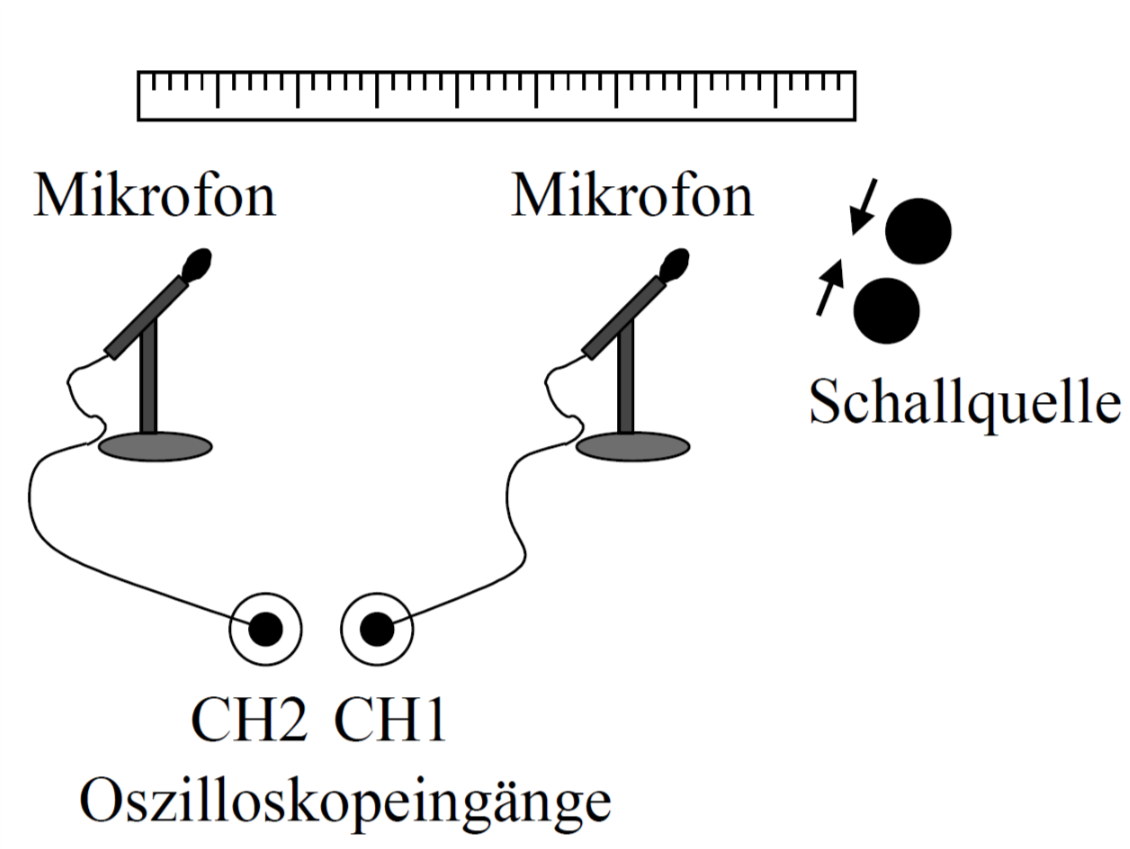
\includegraphics[width=0.5\textwidth]{Bilder/Versuchsaufbau1.png}
\caption{Bestimmung der Schallgeschwindigkeit in Luft durch Laufzeitmessung}
\label{fig:versuch1}
\end{center}
\end{figure}

\subsection{Bestimmung der Schallgeschwindigkeit in Festkörpern}
Im zweiten Versuch soll -- ebenfalls durch Laufzeitmessung -- die Schallgeschwindigkeit in Festkörpern (in diesem Fall in Form von Stäben) bestimmt werden. Hierzu wird (siehe Abb. \ref{fig:versuch2} mit Hilfe eines Piezoelektrischen Körpers, angeschlossen an ein Oszilloskop, der Abstand zwischen zwei Maxima der (longitudinalen) Auslenkungen und damit die Zeit, die ein Schallimpuls für die doppelte Länge des Stabes benötigt. Der Impuls wird durch einen leichten Schlag auf den Stab erzeugt. Auch für diesen Versuch werden mehrere Messreihen, sowie der Abstand von jeweils mehreren Maxima, gemessen.\\
Zudem wird die Schallgeschwindigkeit für drei verschiedene Materialien ermittelt.

\begin{figure}
\begin{center}
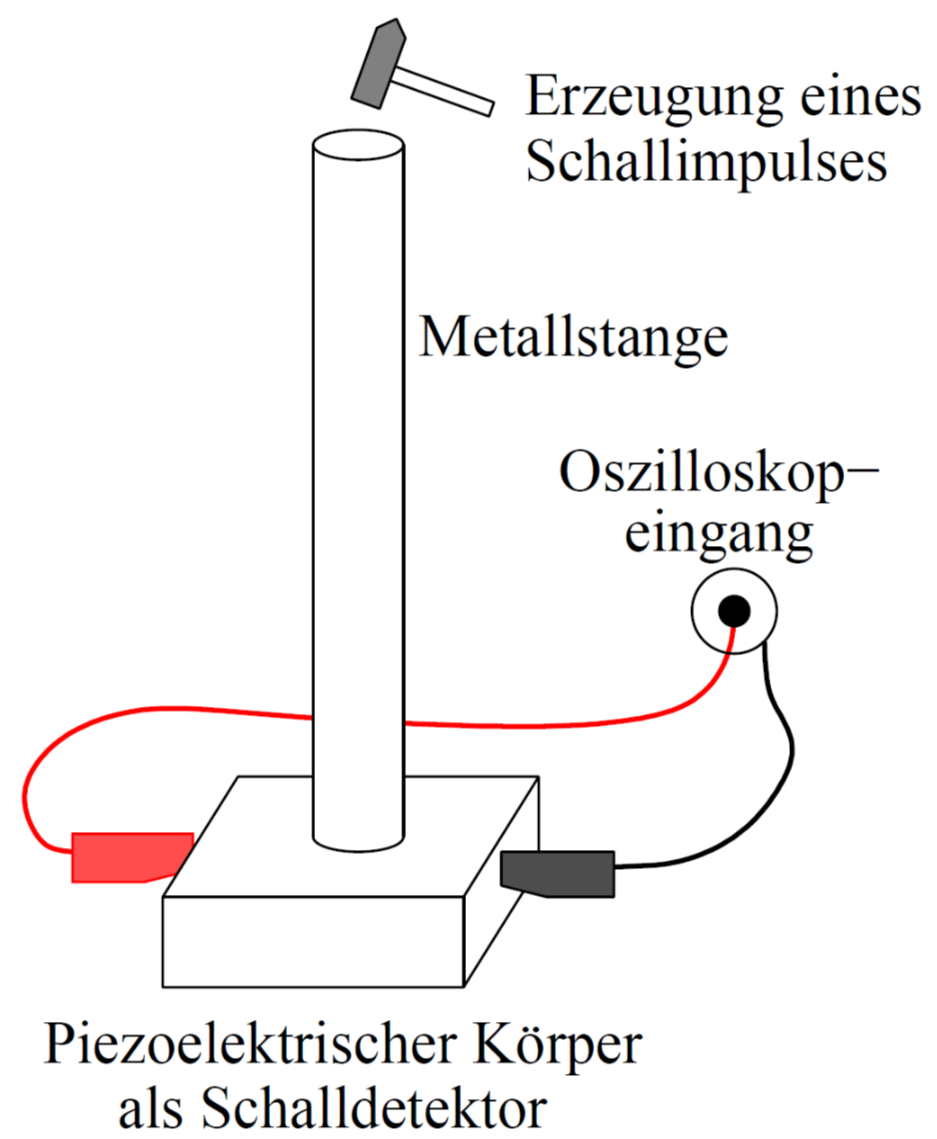
\includegraphics[width=0.3\textwidth]{Bilder/Versuchsaufbau2.png}
\caption{Bestimmung der Schallgeschwindigkeit in Festkörpern durch Laufzeitmessung}
\label{fig:versuch2}
\end{center}
\end{figure}

\subsection{Bestimmung der Schallgeschwindigkeit über stehende Wellen}
In einer Luftsäule wird mit einem Frequenzgenerator eine feste Frequenz angeregt. Mithilfe des in Abbildung \ref{fig:aufgabe3} dargestellten verschiebbaren Stempels wird die Länge der Luftsäule variiert. Es werden die Längen der Luftsäule gemessen, für die eine stehende Welle erzeugt wird, also für die eine Resonanz beobachtet wird. Für drei verschiedene Frequenzen werden möglichst viele Längen der Luftsäule (mit Resonanz) gemessen. Die Messung erfolgt jeweils einmal für eine Verlängerung sowie für eine Verkürzung, sodass zwei Werte für die (theoretisch) gleiche Länge existieren, sodass ein besserer Mittelwert gebildet werden kann. Mithilfe der Gleichung \ref{eq:speedFreq} kann somit die Schallgeschwindigkeit für jeden der ermittelten Längen und der zugehörigen Frequenz berechnet werden.


\begin{figure}
\begin{center}
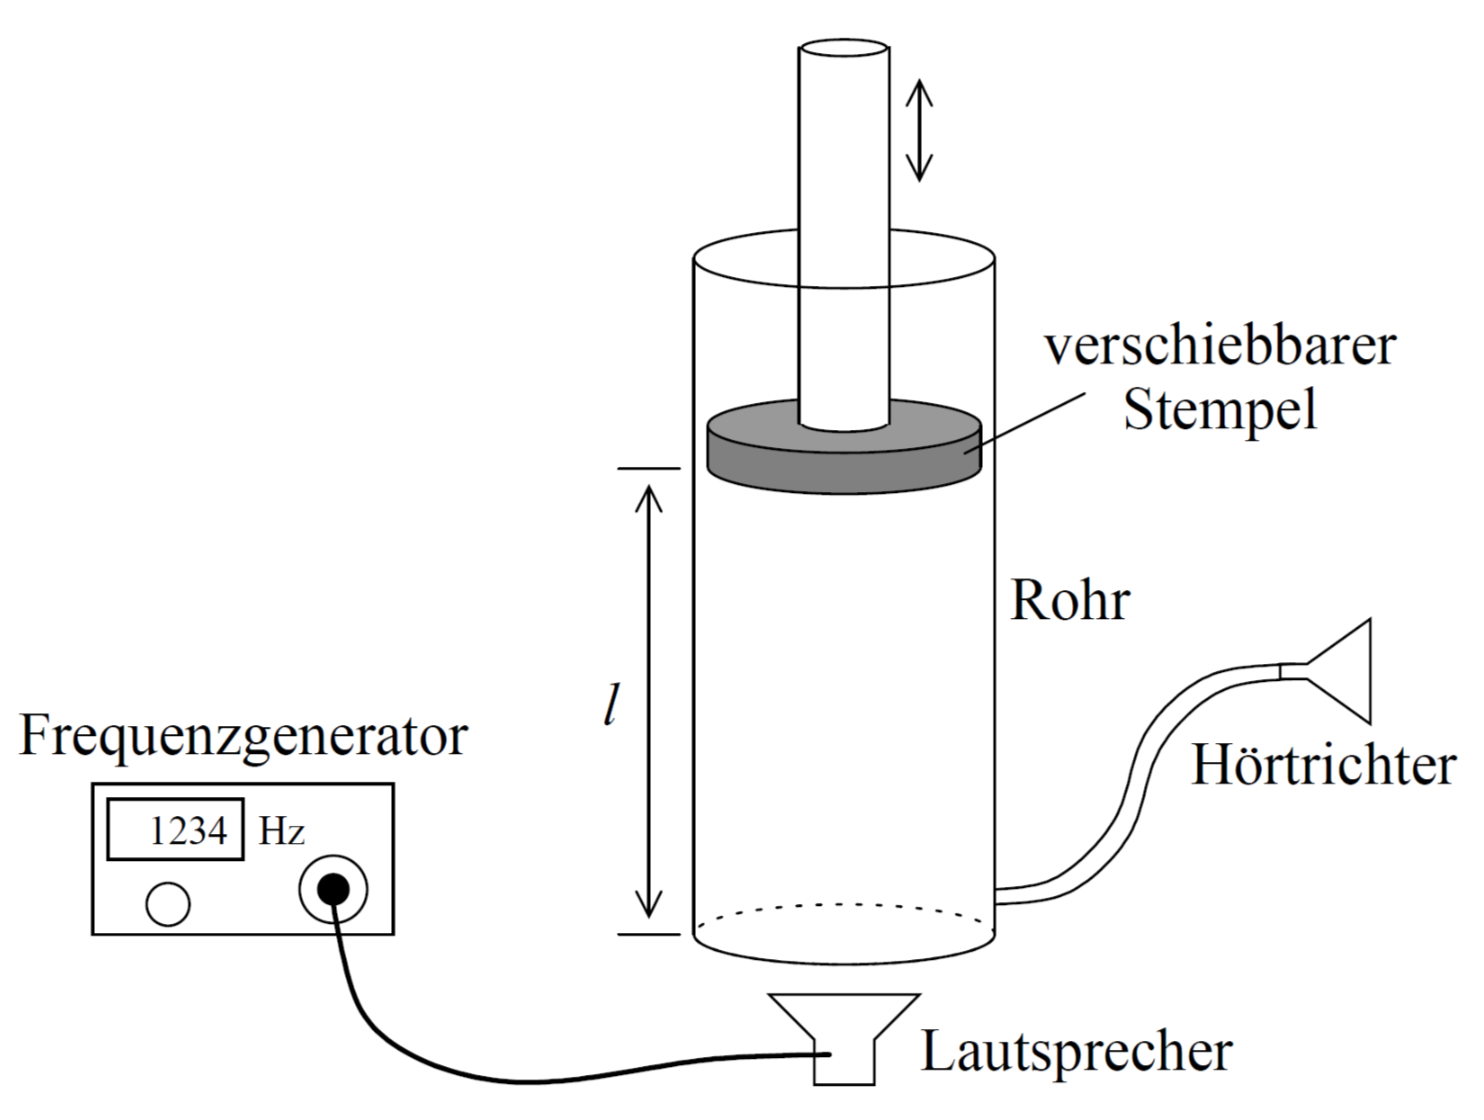
\includegraphics[width=0.3\textwidth]{Bilder/Versuchsaufbau3.png}
\caption{Bestimmung der Schallgeschwindigkeit über stehende Wellen}
\label{fig:versuch3}
\end{center}
\end{figure}


